\documentclass{tufte-handout}

\title{Recitation 1, CIS-2166}

\author{David Dobor}

\date{January 15, 2016} % without \date command, current date is supplied

%\geometry{showframe} % display margins for debugging page layout

\usepackage{graphicx} % allow embedded images
  \setkeys{Gin}{width=\linewidth,totalheight=\textheight,keepaspectratio}
  \graphicspath{{graphics/}} % set of paths to search for images
\usepackage{amsmath}  % extended mathematics
\usepackage{booktabs} % book-quality tables
\usepackage{units}    % non-stacked fractions and better unit spacing
\usepackage{multicol} % multiple column layout facilities
\usepackage{lipsum}   % filler text
\usepackage{fancyvrb} % extended verbatim environments
  \fvset{fontsize=\normalsize}% default font size for fancy-verbatim environments

% Standardize command font styles and environments
\newcommand{\doccmd}[1]{\texttt{\textbackslash#1}}% command name -- adds backslash automatically
\newcommand{\docopt}[1]{\ensuremath{\langle}\textrm{\textit{#1}}\ensuremath{\rangle}}% optional command argument
\newcommand{\docarg}[1]{\textrm{\textit{#1}}}% (required) command argument
\newcommand{\docenv}[1]{\textsf{#1}}% environment name
\newcommand{\docpkg}[1]{\texttt{#1}}% package name
\newcommand{\doccls}[1]{\texttt{#1}}% document class name
\newcommand{\docclsopt}[1]{\texttt{#1}}% document class option name
\newenvironment{docspec}{\begin{quote}\noindent}{\end{quote}}% command specification environment


\usepackage{listings}
\usepackage{color}

\definecolor{dkgreen}{rgb}{0,0.6,0}
\definecolor{gray}{rgb}{0.5,0.5,0.5}
\definecolor{mauve}{rgb}{0.58,0,0.82}

\lstset{frame=tb,
  language=matlab,
  aboveskip=3mm,
  belowskip=3mm,
  showstringspaces=false,
  columns=flexible,
  basicstyle={\small\ttfamily},
  numbers=none,
  numberstyle=\tiny\color{gray},
  keywordstyle=\color{blue},
  commentstyle=\color{dkgreen},
  stringstyle=\color{mauve},
  breaklines=true,
  breakatwhitespace=true,
  tabsize=3
}



\begin{document}

\maketitle% this prints the handout title, author, and date

\begin{abstract}
\noindent
Section 3.2 of Rosen's textbook contains an in-depth discussion of the asymptotic notation.
This note is intended to complement the discussion in the book and may be useful
to ease your understanding of that section. Some example problems and 
their solutions, similar to the ones you'll see on your homework, can 
be found at the end of this note. We will see more examples in following recitations.\end{abstract}


\section{Why use Big-O?}

Suppose you're writing a program that manages inventory for some nation-wide chain
of stores and that every night your job is to process the changes that occured in the inventory 
during that day. 
Suppose it takes about $10, 000  \ ms$ for your program to read in the data from the disk and about 
$10 \ ms$ to process each item in the inventory. If you have $n$ items in the inventory then 
the running time of your program may be represented by:
$$
T(n) = 10, 000 + 10 n
$$




For large $n$, the run-time of your program will be "dominated" by the second term: the time to
read in the data (10 000 $ms$) will become negligible compared to the time it takes to process a 
large amount of inventory items.

In asymptotic analysis we want to abstract away from $T(n)$ the details that do not matter 
in the long run, like the time it takes to read in the data in this example, or the time it takes to process
an individual item. These will vary depending on whether you are running your program on a modern super-computer
or on a desktop from the 80-s that is still stashed away in your parents' garage. We just want to draw some general 
conclusions about the running time of the program you wrote. 

To help reason about $T(n)$, we introduce another
function, $f(n)$, that is simpler than $T(n)$.  We use $f(n)$ for an upper
bound on $T(n)$. This $f(n)$ will enable us to draw conclusions about how fast the inventory processing
algorithm runs, without letting the details get in the way.

\bigskip
Here's a definition of Big-O that is slightly less formal than what the book has:

\bigskip
\newthought{Definition:} We say that $T(n)$ is Big-O of $f(n)$ and write $T(n) \in O(f(n))$ if and only if
$$
T(n) \leq C f(n) \text{ \ whenever } n \text{ is big for some large constant } C 
$$

\bigskip
Well, but what is "big $n$"? Answer: big enough to have the first function, $T(n)$, "fit below" the second one, $f(n)$. 
We'll look at an example in a second. We'll give this "big enough $n$" a name - we'll call it $k$, as the textbook does.
And what is "large enough $C$"? The answer is the same. \emph{And} we get to choose $C$. 

\bigskip
That is, we get to choose the constants $C$ and $k$ such that 
$$
T(n) \leq C f(n) \ \ \ \text{ whenever } \ n > k
$$

\bigskip
If we can identify such $C$ and $k$, then we say that $T(n) \in O(f(n))$; Otherwise, if we can prove that no such $C$ and $k$ exist, then we say that $T(n) \not\in O(f(n))$

\bigskip
Whenever you see $T(n) \in O(f(n))$, it may be helpful to think: "$T(n)$ is smaller than $f(n)$" or that 
"$f(n)$ dominates $T(n)$". 


\bigskip
(\emph{As an aside}, note that we do not usually write that $T(n) = O(f(n))$. We 
instead think of $f(n)$ as being a member - or being "like" other members - of a \emph{set} of functions 
denoted by $O(f(n))$. 
However, people often use the "=" sign, and that is something to be aware of. We'll stick with the "$\in$" sign in our discussions.)

\section{Examples}

\newthought{Example $0$:} Consider comparing $T(n) = 10 + 2n$ to 
$f(n) = n$. We want to see if $f(n)$ will dominate $T(n)$ for large enough $n$. That is, will 
the plot of $f(n)$ be above the plot of $T(n)$ if
we were to plot the two functions? In fact, let's plot them.

Let's set the constant $C$ in the above definition to $1$ and see what the plots look like. 
If you are inclined to use Matlab (not required for this course), here's how to do it.



\bigskip 

\begin{lstlisting}
n = linspace(0,20,100);
T = 10 + 2*n;
f = 1*n;

figure(1)
plot(n,T, 'linewidth', 2, 'color', 'g')
xlim([0 20])
ylim([0 50])
hold on
plot(n,f, 'linewidth', 2, 'color', 'b')
legend('T(n) = 10 + 2 n', 'f(n) = n', 'location', 'northwest')
\end{lstlisting}

\begin{figure}
  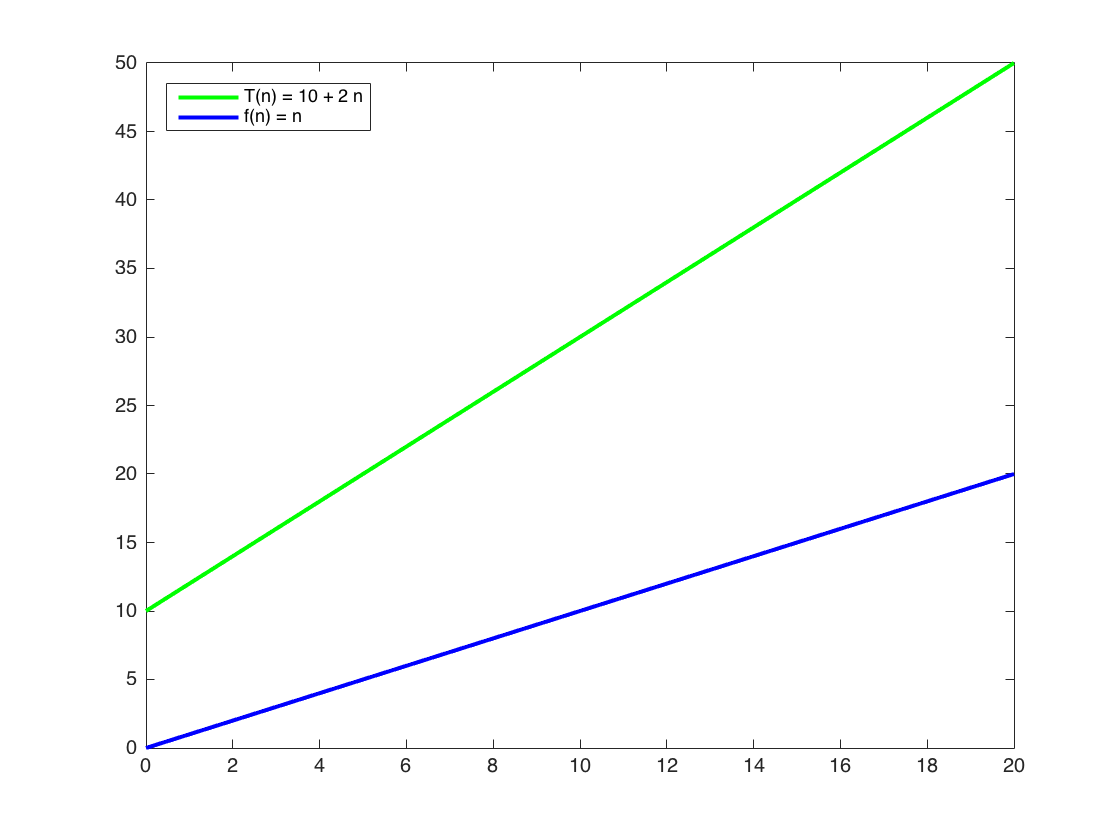
\includegraphics{BigO1.png}
%  \checkparity This is an \pageparity\ page.%
  \caption{Here $T(n)$ dominates $f(n)$ everywhere, meaning that the plot of $f(n)$ fits entirely under the plot of $T(n)$.}
  \label{fig:textfig}
  %\zsavepos{pos:textfig}
  \setfloatalignment{b}
\end{figure}

\pagebreak
At first it may appear to you that since $f(n)$ is below $T(n)$, we can't really claim that $T(n) \in O(f(n))$. 

But recall from the definition that we get to choose $C$. In the above figure, $C$ is $1$. 
Now consider setting $C$ to something like 5. We then can have $f(n)$ dominate $T(n)$. 

\bigskip 

 
 \begin{lstlisting}
f = 5*n; 
plot(n,T, 'linewidth', 2, 'color', 'g')
xlim([0 20])
ylim([0 50])
hold on
plot(n,f, 'linewidth', 2, 'color', 'b')
legend('T(n) = 10 + 2 n', 'f(n) = 5 n', 'location', 'northwest')
\end{lstlisting}

\begin{figure}
  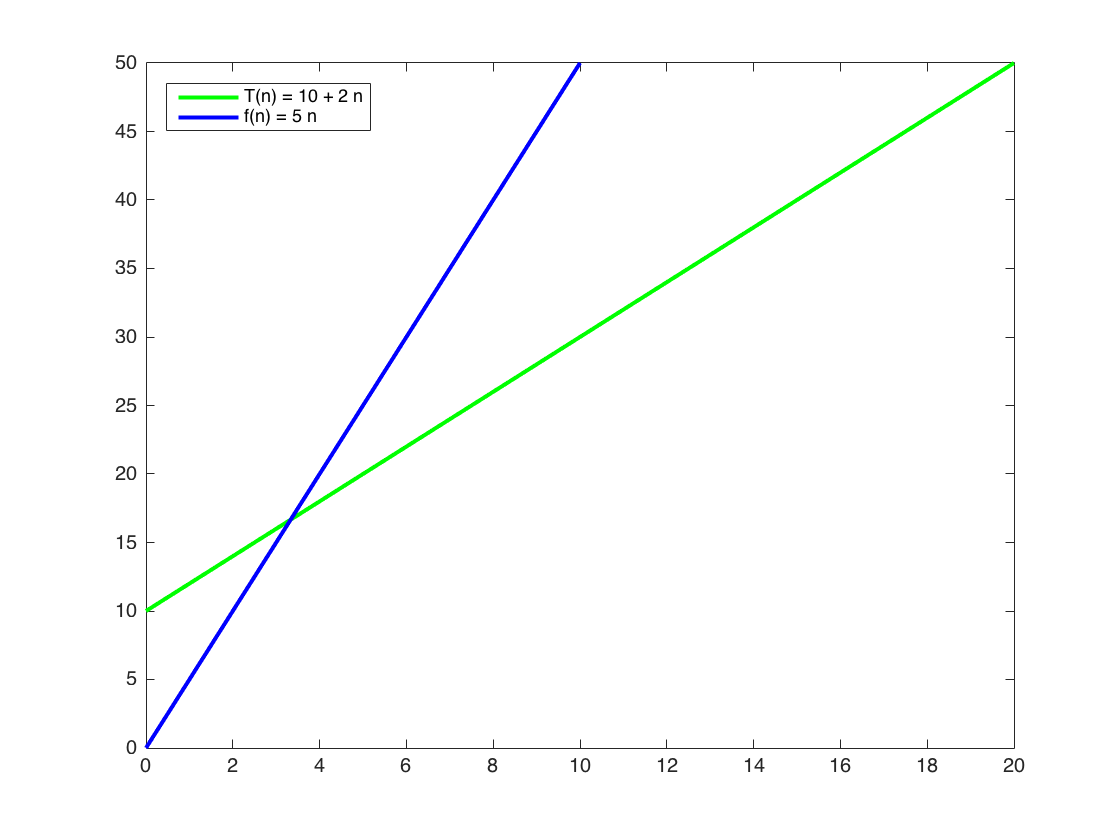
\includegraphics{BigO2.png}
%  \checkparity This is an \pageparity\ page.%
  \caption{Here $f(n)$ begins to dominate $T(n)$ after a certain point.}
  \label{fig:textfig}
  %\zsavepos{pos:textfig}
  \setfloatalignment{b}
\end{figure}


\bigskip
So now we see that after a certain point $f$ begins to dominate $T$ instead (what is that 
point?). Now it should be clearer how $f$ and $T$ in this example fit the Big-O definition.

\bigskip
Now consider other examples similar to what you will find in your homework. The trick to solving
these problems is to explicitly identify the constants $C$ and $k$ that fit the above definition. 
We rely on the mathematical fact that $\log(n) \leq n$ for $n \geq 1$.

\newthought{Example 1:} 

$5 n^2 + 3 n \log n + 2 n + 5 $ \ is  \ $ O(n^2)$

\newthought{Justification:}  $5 n^2 + 3 n \log n + 2 n + 5 \leq (5 + 3 + 2 + 5) n^2  = C n^2 $ for 
$C = 15$ when $n \geq k = 1$

\newthought{Example 2:} 

$20 n^3 + 10 n \log n + 5 $ \ is  \ $ O(n^3)$

\newthought{Justification:}  $5 n^2 + 3 n \log n + 2 n + 5 \leq 35 n^2$ for $n \geq k = 1$


\newthought{Example 3:} 

$3n \log n + 5 $ \ is  \ $ O(\log n)$

\newthought{Justification:}  $3n \log n + 5  \leq 8 \log n$ for $n \geq n_0 = 2$. Note that 
$\log n$ is zero for $n = 1$. That is why we use $k = 2$ here.


\newthought{Example 4:} 

$2^{n+2}$ \ is  \ $O(2^n)$

\newthought{Justification:} $2^{n+2} = 2^n \cdot 2^2 = 4 \cdot 2^n$, so we can take $C = 4$ and $k = 1$ in this case. 


\newthought{Example 5:} 

$2 n + 100 \log n$ \ is  \ $O(n)$

\newthought{Justification:} $2 n + 100 \log n \leq 102 n$ for $n \geq 1$,  so we can take $C = 102$ and $k = 1$ in this case. 



\end{document}



\emph{Big-O} notation is used to represent upper bounds on functions. 
We think of Big-O notation as an abstract relation between functions. A function
may be the worst case running time of a program, but it doesn't have to be. 


















